
%% Creator David Li
% Modified matlab xsl latex template file to suit needs
% Use find and replace 
%		\ensuremath with ''
%		
%	    \{ with { and \} with }
% This LaTeX was auto-generated from an M-file by MATLAB.
% To make changes, update the M-file and republish this document.

\documentclass{article}

% Wait until lwarp has better support for listings, or just shove the listings under a tcolourbox, because the matlab output (under tcolourbox)
%  looks fine at the moment.
%\usepackage[
% HomeHTMLFilename=index,     % Filename of the homepage.
%HTMLFilename={node-},       % Filename prefix of other pages.
% IndexLanguage=english,      % Language for xindy index, glossary.
% latexmk,                    % Use latexmk to compile.
%   OSWindows,                  % Force Windows. (Usually automatic.)
% mathjax,                    % Use MathJax to display math.
% ]{lwarp}

\title{Assignment 1}
\author{David Li}
\date{\today}
\usepackage[utf8]{inputenc}
\usepackage{graphicx}
\usepackage{epstopdf}
\usepackage{color}
\usepackage{xcolor}
\usepackage{amsmath}
\usepackage[ocgcolorlinks]{hyperref}
\usepackage{bookmark}
\usepackage[hmargin=2cm,vmargin=2.5cm]{geometry}
\usepackage{fancyhdr}
\usepackage{booktabs}
\sloppy
\definecolor{lightgray}{gray}{0.5}
% \definecolor{myText}{HTML}{2B2B2B}
\definecolor{fontColor}{HTML}{171717}
\setlength{\parindent}{0pt}

\makeindex

\usepackage{listings}
\definecolor{mygreen}{RGB}{28,172,0} % color values Red, Green, Blue
\definecolor{mylilas}{RGB}{170,55,241}
\lstset{language=Matlab,%
	%basicstyle=\color{red},
	breaklines=true,%
	morekeywords={matlab2tikz},
	keywordstyle=\color{blue},%
	morekeywords=[2]{1}, keywordstyle=[2]{\color{black}},
	identifierstyle=\color{black},%
	stringstyle=\color{mylilas},
	commentstyle=\color{mygreen},%
	showstringspaces=false,%without this there will be a symbol in the places where there is a space
	%numbers=left,%
	%numberstyle={\tiny \color{black}},% size of the numbers
	%numbersep=9pt, % this defines how far the numbers are from the text
	emph=[1]{for,end,break},emphstyle=[1]\color{red}, %some words to emphasise
	%emph=[2]{word1,word2}, emphstyle=[2]{style},  
    captionpos=b,
    caption={Matlab Code Snippet:},
}
\usepackage{tcolorbox}
\tcbuselibrary{listings}
\tcbuselibrary{breakable}





\newtcblisting[auto counter,number within=section*]{matlaboutput}[2][]{sharp corners, breakable,
    fonttitle=\bfseries,colback=white, colframe=black!90, listing only, 
    listing options={language=Matlab, showstringspaces=false, breakatwhitespace=true, breaklines=true, tabsize=4}, 
    title=Matlab Output \thetcbcounter: #1} 

\usepackage{enumitem}
\begin{document}

\noindent \large{\textbf{ELEC 460 --- Assignment 1}\hfill Name: \textbf{David Li}, \hfill  Student Number: \textbf{V00818631}} \hrule
%\textbf{Due Date:} \today \hfill Student Number: \textbf{V00818631}

    
    
\section*{ELEC 300 reference document,}
      \begin{par}
going through circuit analysis with matlab to create and document useful features. This is the document that will be published
\end{par} \vspace{1em}

\tableofcontents
\newpage
\begin{enumerate}
\setlength{\itemsep}{-1ex}
   \item Another list
   \item lists
   \item trades
\end{enumerate}
\begin{lstlisting}[language = Matlab,frame=single,caption={}]
format compact
format rational
\end{lstlisting}


\begin{description}[style=nextline] %% Style for this list only.
	\item[Turquoise] Medium to long labels force the description to the next line.
	\item[Red] Short labels still have the description on the same line.
	\item[Red~~~] To force the description to the next line, pad the label with \textasciitilde.
\end{description}

\subsection*{Introduction}
\addcontentsline{toc}{subsection}{Introduction}
\phantomsection


        \begin{par}
testing things out, what exactly is the introduction section
\end{par} \vspace{1em}


\subsection*{SECTION TITLE WITHOUT SECTION BREAK}
\addcontentsline{toc}{subsection}{SECTION TITLE WITHOUT SECTION BREAK}
\phantomsection


        \begin{par}
DESCRIPTIVE TEXT
\end{par} \vspace{1em}
\begin{lstlisting}[language = Matlab,frame=single,caption={}]
G=[1 0 0 0 0;...
 -1/3 5/6 -1/3 0 0;...
 0 -1/3 13/30 19/60 -19/60;...
 0 -10/3 1 -1 0;...
 0 0 -1/10 -19/60 37/60]
I=[12 0 0 0 0]'
V=G\I
fprintf('\n');...
 fprintf('v1 = %7.2f V \n',V(1));...
 fprintf('v2 = %7.2f V \n',V(2));...
 fprintf('v3 = %7.2f V \n',V(3));...
 fprintf('v4 = %7.2f V \n',V(4));...
 fprintf('v5 = %7.2f V \n',V(5));...
 fprintf('\n'); fprintf('\n')


z1=4-j*6; z2=2+j*3; z3=8-j*3; % Define z1, z2 and z3
Z=[1/z1+1/z2 -1/z2; -1/z2 1/z2+1/z3]; % Elements of matrix Z
I=[5 -10]'; % Column vector I
V=Z\I; Va=V(1,1); Vb=V(2,1); Vab=Va-Vb; % Va = V(1), Vb = V(2) are also acceptable
% With f p r i n t f only the real part of each parameter is processed so we will use di s p
fprintf(' \n'); disp('Va = '); disp(Va); disp('Vb = '); disp(Vb); disp('Vab = '); disp(Vab);
fprintf(' \n');

Z=[1 0 0; -(4-j*6) 14-j*6 -(8-j*3); 0 0 1];
V=[5 0 10]';
I=Z\V; i1=I(1); i2=I(2); i3=I(3); fprintf(' \n');
disp('i1 = '); disp(i1); disp('i2 = '); disp(i2); disp('i3 = '); disp(i3);

z1=4-6j; z2=2+3j; z3=8-3j; Is=5; i1=z1*Is/(z1+z2+z3);...
i1, magI1=abs(i1), phaseI1=angle(i1)*180/pi, v1=-3j*i1,...
magV1=abs(v1), phaseV1=angle(v1)*180/pi,...
Is2=-10; i2=(z1+z2)*Is2/(z1+z2+z3); magI2=abs(i2), phaseI2=angle(i2)*180/pi,...
v2=-3j*i2, magV2=abs(v2), phaseV1=angle(v2)*180/pi,...
vC=v1+v2, magvC=abs(vC), phasevC=angle(vC)*180/pi
\end{lstlisting}

\begin{quote}
 \begin{verbatim}{}G =
       1              0              0              0              0       
      -1/3            5/6           -1/3            0              0       
       0             -1/3           13/30          19/60         -19/60    
       0            -10/3            1             -1              0       
       0              0             -1/10         -19/60          37/60    
I =
      12       
       0       
       0       
       0       
       0       
V =
      12       
     952/73    
    1504/73    
   -5008/219   
   -1840/219   

v1 =   12.00 V 
v2 =   13.04 V 
v3 =   20.60 V 
v4 =  -22.87 V 
v5 =   -8.40 V 


 
Va = 
    -120/29     +  570/29i   
Vb = 
    -650/29     -   30/29i   
Vab = 
     530/29     +  600/29i   
 
 
i1 = 
       5       
i2 = 
     220/29     -   30/29i   
i3 = 
      10       
i1 =
     115/58     -   75/58i   
magI1 =
    1283/542   
phaseI1 =
  -16059/485   
v1 =
    -225/58     -  345/58i   
magV1 =
    3359/473   
phaseV1 =
  -59709/485   
magI2 =
    3607/819   
phaseI2 =
   28438/161   
v2 =
      45/58     +  765/58i   
magV2 =
    3607/273   
phaseV1 =
   13948/161   
vC =
     -90/29     +  210/29i   
magvC =
     583/74    
phasevC =
   15961/141   
\end{verbatim}
    \end{quote}

\subsection*{Another Section}

\begin{description}[style=nextline] %% Style for this list only.
	\item[Turquoise] Medium to long labels force the description to the next line.
	\item[Red] Short labels still have the description on the same line.
	\item[Red~~~] To force the description to the next line, pad the label with \textasciitilde.
\end{description}
\addcontentsline{toc}{subsection}{Another Section}
\phantomsection

\begin{verbatim}{}G =
1              0              0              0              0       
-1/3            5/6           -1/3            0              0       
0             -1/3           13/30          19/60         -19/60    
0            -10/3            1             -1              0       
0              0             -1/10         -19/60          37/60    
I =
12       
0       
0       
0       
0       
V =
12       
952/73    
1504/73    
-5008/219   
-1840/219   

v1 =   12.00 V 
v2 =   13.04 V 
v3 =   20.60 V 
v4 =  -22.87 V 
v5 =   -8.40 V 



Va = 
-120/29     +  570/29i   
Vb = 
-650/29     -   30/29i   
Vab = 
530/29     +  600/29i   


i1 = 
5       
i2 = 
220/29     -   30/29i   
i3 = 
10       
i1 =
115/58     -   75/58i   
magI1 =
1283/542   
phaseI1 =
-16059/485   
v1 =
-225/58     -  345/58i   
magV1 =
3359/473   
phaseV1 =
-59709/485   
magI2 =
3607/819   
phaseI2 =
28438/161   
v2 =
45/58     +  765/58i   
magV2 =
3607/273   
phaseV1 =
13948/161   
vC =
-90/29     +  210/29i   
magvC =
583/74    
phasevC =
15961/141   
\end{verbatim}


        \begin{lstlisting}[language = Matlab,frame=single,caption={}]
clear all
% Enter the non-zero values of the G matrix
G(1,1)=1;
G(2,1)=-1/2;
G(2,2)=1/2-1/5j+1/3j;
G(2,3)=-1/3j;
G(3,2)=-1/3j;
G(3,3)=1/3j+1/5;
%
% Enter all values of the I matrix
I=[1 0 0]';
%
% Compute node voltages
V=G\I;
%
VR1=V(1)-V(2);
VL=V(2)-V(3);
% Compute magnitudes and phase angles of voltages
magV1=abs(V(1)); magV2=abs(V(2)); magV3=abs(V(3));
phaseV1=angle(V(1))*180/pi; phaseV2=angle(V(2))*180/pi; phaseV3=angle(V(3))*180/pi;
magVR1=abs(VR1); phaseVR1=angle(VR1)*180/pi;
magVL=abs(VL); phaseVL=angle(VL)*180/pi;
%
% Denote radian frequency as w and plot wt for 0 to 2*pi range
wt=linspace(0,2*pi);
V1=magV1*cos(wt-phaseV1);
V2=magV2*cos(wt-phaseV2);
V3=magV3*cos(wt-phaseV3);
VR1t=magVR1*cos(wt-phaseVR1);
VLt=magVL*cos(wt-phaseVL);
%
% Convert wt to degrees
deg=wt*180/pi;
%
% Print phasor voltages, magnitudes, and phase angles
fprintf(' \n');
% With f p r i n t f only the real part of each parameter is processed so we will use d i s p
disp('V1 = '); disp(V(1)); disp('V2 = '); disp(V(2)); disp('V3 = '); disp(V(3));
disp('VR1 = '); disp(VR1); disp('VL = '); disp(VL);
fprintf('magV1 = %4.2f V \t', magV1); fprintf('magV2 = %4.2f V \t', magV2);
fprintf('magV3 = %4.2f V', magV3); fprintf(' \n'); fprintf(' \n');
fprintf('phaseV1 = %4.2f deg \t', phaseV1);
fprintf('phaseV2 = %4.2f deg \t', phaseV2); fprintf('phaseV3 = %4.2f deg', phaseV3);
fprintf(' \n'); fprintf(' \n');
fprintf('magVR1 = %4.2f V \t', magVR1); fprintf('phaseVR1 = %4.2f deg ', phaseVR1);
fprintf(' \n'); fprintf(' \n');
fprintf('magVL = %4.2f V \t', abs(VL)); fprintf('phaseVL = %4.2f deg ', phaseVL);
fprintf(' \n');
%
plot(deg,V1,deg,V2,deg,V3,deg,VR1t,deg,VLt)
fprintf(' \n');
\end{lstlisting}

         
 \begin{matlaboutput}{} 
V1 = 
       1       
V2 = 
     550/733    -   95/733i  
V3 = 
     725/1466   -  625/1466i 
VR1 = 
     183/733    +   95/733i  
VL = 
     375/1466   +  435/1466i 
magV1 = 1.00 V 	magV2 = 0.76 V 	magV3 = 0.65 V 
 
phaseV1 = 0.00 deg 	phaseV2 = -9.80 deg 	phaseV3 = -40.76 deg 
 
magVR1 = 0.28 V 	phaseVR1 = 27.43 deg  
 
magVL = 0.39 V 	phaseVL = 49.24 deg  
 
\end{matlaboutput}
    
    
    \begin{verse}
    	Anime wins again
    \end{verse}

\begin{quote}
	Anime loses again.
\end{quote}
\begin{figure}
	\centering
	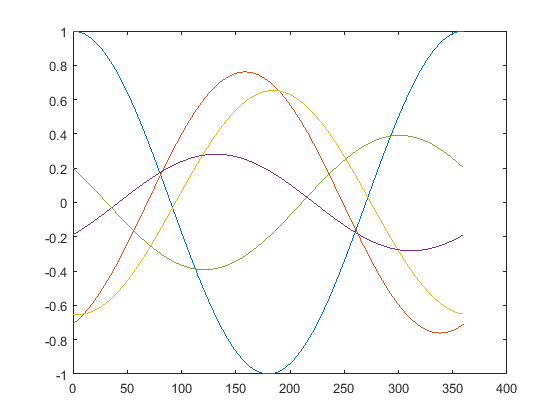
\includegraphics [width=0.7\linewidth]{ReferenceDocument_01.png}
	\caption{$ReferenceDocument_01.png$}
	%\caption{}
	% Alternative is to typeset the caption myself, which makes more sense to me.
	% \label{$fig:ReferenceDocument_01.png$}
\end{figure}
\begin{par}
$$H = w_x + 5$$
\end{par} \vspace{1em}
\begin{par}
\href{http://www.mathworks.com}{MathWorks}
\end{par} \vspace{1em}
\begin{par}
\href{matlab:FUNCTION}{DISPLAYED TEXT}
\end{par} \vspace{1em}



\end{document}
    
